\chapter{恒星作为量子光源}
\label{chap:10}

\begin{chapteropening}
恒星很适合作为第一批量子天文学目标。光球连续谱近似热光，亮星有足够光子率，角直径在毫角秒量级；强度干涉可以直接测 \(|V|^2\)，不要求望远镜之间保持光学相位。但恒星表面并非完美圆盘。边缘昏暗、快速自转、星斑、双星、脉动和星风都会把表面亮度分布写进可见度曲线。前面建立的相干函数、事件表和 Fisher 信息，在恒星问题中对应半径、有效温度、旋转和距离标尺 \citep{1956Natur.177...27B,1967MNRAS.137..375H,1967MNRAS.137..393H,1974MNRAS.167..121H,1974iiia.book.....H,2020NatAs...4.1164A,2024MNRAS.529.4387A}。
\end{chapteropening}

\section{为什么恒星是最稳的标定场}

恒星光球在局部热平衡下发出近似热辐射。单个相干模式的热光有 \(g^{(2)}(0)=2\)，但真实恒星观测混合了大量空间、偏振、频率和时间模式，实际可见的 \(g^{(2)}(0)-1\) 很小。Vega photon-counting 强度干涉实验在零基线测得 \(\langle g^{(2)}\rangle=1.0034\pm0.0008\)，在约 \(2~{\rm km}\) 基线上没有显著相关，结果与 Vega 约 \(3.3~{\rm mas}\) 的角直径相容 \citep{2021MNRAS.506.1585Z}。这是第 \ref{chap:09} 章模式数稀释在恒星上的实际版本。

强度干涉测量的是两台望远镜光强涨落的相关。对热光，校准后的零延迟相关与复可见度满足
\begin{equation}
  g^{(2)}_{ij}(0)-1 = |\gamma_{ij}|^2 \simeq |V(u_{ij},v_{ij})|^2 .
  \label{eq:ch10-g2-visibility}
\end{equation}
\begin{formulaexplain}
\(g^{(2)}_{ij}(0)\) 是望远镜 \(i,j\) 的零延迟强度相关；\(\gamma_{ij}\) 是复相干度，\(V\) 是归一化可见度。热光强度干涉把相关超额变成天空亮度 Fourier 模平方。
\end{formulaexplain}
\(\gamma_{ij}\) 是两台望远镜之间的复相干度，\((u,v)={\bf B}_\perp/\lambda\) 是投影基线除以波长，单位是波长数。观测中左边来自延迟直方图、时间移位背景扣除和归一化相关；右边是天空亮度分布的 Fourier 模平方。相位丢失意味着 \(|V|^2\) 对镜像和整体平移不敏感，但角直径、轴比、双星间距和某些对称结构仍可精确测量。

基线和角尺度由同一个比例给出：
\begin{equation}
  B\sim\frac{\lambda}{\theta}
  \simeq 103~{\rm m}
  \left(\frac{\lambda}{500~{\rm nm}}\right)
  \left(\frac{\theta}{1~{\rm mas}}\right)^{-1}.
  \label{eq:ch10-baseline-scale}
\end{equation}
\begin{formulaexplain}
\(B\) 是基线长度，\(\lambda\) 是波长，\(\theta\) 是目标角尺度。这个比例说明可见光百米基线对应毫角秒恒星，公里基线才进入更小表面结构。
\end{formulaexplain}
一个 \(1~{\rm mas}\) 的恒星在可见光需要百米基线开始明显分辨；\(0.1~{\rm mas}\) 的表面结构需要公里量级基线。Narrabri 强度干涉仪用 \(10\)--\(188~{\rm m}\) 基线和两个 \(6.7~{\rm m}\) 反射面测量了 32 颗亮星角直径；现代 VERITAS、MAGIC 和未来 CTA 类型阵列用 \(>10~{\rm m}\) 级 Cherenkov 望远镜、大面积收光和数字相关器重新打开了这个参数空间 \citep{1974MNRAS.167..121H,2012NewAR..56..143D,2020NatAs...4.1164A,2024MNRAS.529.4387A}。

强度干涉的信噪比标度已在式 \eqref{eq:ch05-snr} 给出。放到恒星样本上，它的主要含义很直接：光子率越高、电子带宽越大、积分越久，\(|V|^2\) 的误差越小；背景、死时间、有限时间分辨率和系统协方差则决定这种统计增益会在哪里停止。因此第一批样本自然偏向亮、热、蓝、角直径在百米级基线可分辨的恒星 \citep{2013MNRAS.430.3187R,2020NatAs...4.1164A}。

\section{怎样从平方可见度读出角直径和温度}

从数据到半径的第一步，是把恒星暂时当成一个只有角直径的圆盘。最基础的恒星模型仍是第 \ref{chap:05} 章的均匀圆盘，使用式 \eqref{eq:ch05-uniform-disk}。这里 \(B\) 是投影基线，\(\lambda\) 是有效波长，\(\theta\) 用弧度；若 \(\theta\) 以 mas 给出，要乘以 \(4.848\times10^{-9}\) 转成弧度。强度干涉拟合的是 \(|V_{\rm UD}|^2\)，复相位已经被平方模取代。第一零点附近对角直径最敏感，但 \(|V|^2\) 太低时系统误差和背景会变得重要，所以实际观测要覆盖短、中、长基线。短基线固定总通量和相关归一化，中等基线给出直径斜率，长基线检查模型是否需要边缘昏暗、扁率或伴星。

\begin{figure}[tbp]
\centering
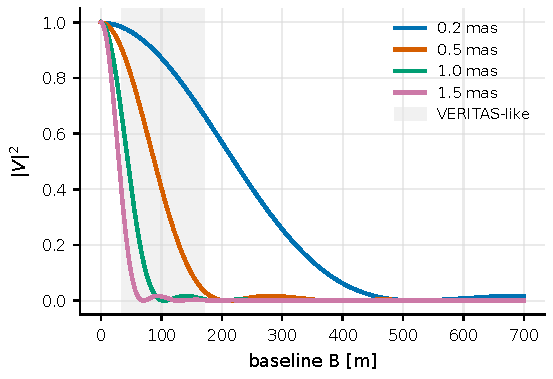
\includegraphics[width=0.82\linewidth]{figures/generated/chapter_10/ch10_stellar_diameter_visibility.pdf}
\caption{均匀圆盘恒星的 \(|V|^2\) 随基线变化。波长取 \(416~{\rm nm}\)，接近 VERITAS SII 的观测波长。角直径越大，可见度下降越快；灰色区域标出 \(35\)--\(170~{\rm m}\) 的 VERITAS 量级投影基线范围，适合测量约 \(0.5\)--\(1.5~{\rm mas}\) 的亮星。}
\label{fig:chapter-10-diameter-visibility}
\end{figure}

角直径和总辐射流量给出有效温度。若 \(F_{\rm bol}\) 是地球处测得的 bolometric flux，单位 \({\rm erg\,s^{-1}\,cm^{-2}}\)，则
\begin{equation}
  F_{\rm bol}=\frac{\theta_{\rm LD}^2}{4}
  \sigma_{\rm SB}T_{\rm eff}^4,
  \qquad
  T_{\rm eff}=
  \left(\frac{4F_{\rm bol}}{\sigma_{\rm SB}\theta_{\rm LD}^2}\right)^{1/4}.
  \label{eq:ch10-teff}
\end{equation}
\begin{formulaexplain}
\(F_{\rm bol}\) 是地球处总辐射流量，\(\theta_{\rm LD}\) 是边缘昏暗角直径，\(\sigma_{\rm SB}\) 是 Stefan--Boltzmann 常数。角直径和总流量共同给出有效温度。
\end{formulaexplain}
\(\theta_{\rm LD}\) 是边缘昏暗角直径，\(\sigma_{\rm SB}\) 是 Stefan--Boltzmann 常数。误差传播为
\begin{equation}
  \left(\frac{\sigma_T}{T_{\rm eff}}\right)^2
  \simeq
  \frac{1}{16}\left(\frac{\sigma_F}{F_{\rm bol}}\right)^2
  +\frac{1}{4}\left(\frac{\sigma_\theta}{\theta_{\rm LD}}\right)^2 .
  \label{eq:ch10-teff-error}
\end{equation}
\begin{formulaexplain}
\(\sigma_T,\sigma_F,\sigma_\theta\) 分别是温度、总流量和角直径误差。因为 \(T_{\rm eff}\propto F_{\rm bol}^{1/4}\theta_{\rm LD}^{-1/2}\)，同等百分比下角直径误差更重要。
\end{formulaexplain}
角直径误差进入系数是 \(1/2\)，常常主导 \(T_{\rm eff}\)。VERITAS 对 \(\beta\) UMa 的 SII 观测得到 \(\theta_{\rm LD}=1.07\pm0.04{\rm(stat)}\pm0.05{\rm(sys)}~{\rm mas}\)，由此给出 \(T_{\rm eff}\simeq9700\pm200\pm200~{\rm K}\)，并可进一步约束 Ursa Major moving group 的年龄 \citep{2024ApJ...966...28A}。

\begin{figure}[tbp]
\centering
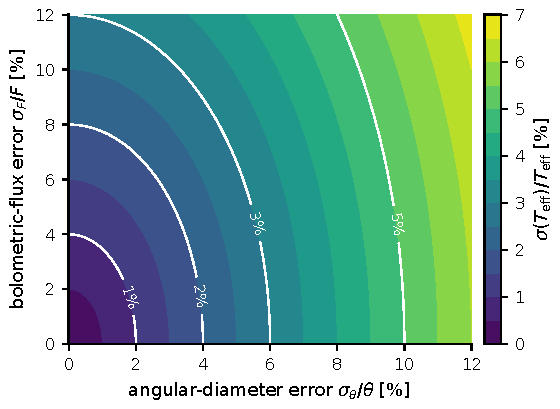
\includegraphics[width=0.78\linewidth]{figures/generated/chapter_10/ch10_teff_error_budget.pdf}
\caption{由 \(F_{\rm bol}\) 和 \(\theta_{\rm LD}\) 推导 \(T_{\rm eff}\) 的误差传播。横轴是角直径相对误差，纵轴是总流量相对误差，颜色给出有效温度相对误差。由于 \(T_{\rm eff}\propto F_{\rm bol}^{1/4}\theta^{-1/2}\)，角直径误差通常比同等百分比的流量误差更重要。}
\label{fig:chapter-10-teff-error}
\end{figure}

\Needspace{13\baselineskip}
若距离 \(d\) 已知，半径和光度为
\begin{equation}
  R=\frac{1}{2}\theta_{\rm LD}d,\qquad
  L=4\pi R^2\sigma_{\rm SB}T_{\rm eff}^4 .
  \label{eq:ch10-radius-luminosity}
\end{equation}
\begin{formulaexplain}
\(R\) 是恒星半径，\(d\) 是距离，\(L\) 是光度。角直径给出天空上的大小，距离把它变成物理半径，再由 Stefan--Boltzmann 定律得到光度。
\end{formulaexplain}
Gaia 视差、干涉角直径和 \(F_{\rm bol}\) 联合后，恒星会落到 HR 图上一个带协方差的区域。这个区域与演化轨道比较给出质量、年龄和混合长度、超调、旋转等模型约束。红外流量法、Mark III/CHARA 等振幅干涉角直径和 SII 角直径在这一层面是互补的标尺 \citep{1977MNRAS.180..177B,1991AJ....101.2207M,1994A&A...282..899B,2003AJ....126.2502M,2005ApJ...626..446R}。

\section{边缘昏暗为什么不是小修正}

真实恒星边缘更暗，因为视线穿过的温度层不同。最简单的线性边缘昏暗模型为
\begin{equation}
  I(\mu)=I(1)\,[1-u_\lambda(1-\mu)],
  \qquad
  \mu=\sqrt{1-r^2}.
  \label{eq:ch10-linear-ld}
\end{equation}
\begin{formulaexplain}
\(I(\mu)\) 是不同视角处的表面亮度；\(\mu\) 是法线与视线夹角余弦，\(r\) 是归一化投影半径，\(u_\lambda\) 是边缘昏暗系数。它把恒星边缘变暗写成一个简化剖面。
\end{formulaexplain}
\(r\) 是投影圆盘半径除以恒星半径，\(\mu\) 是表面法线与视线夹角的余弦，\(u_\lambda\) 是波长相关的边缘昏暗系数。热星在蓝光、冷巨星在分子带、Mira 变量在不同相位都会有不同的 \(I(\mu)\)。现代分析通常从大气模型或 limb-darkening toolkit 生成合成强度分布，再计算可见度；线性 \(u_\lambda\) 更适合做数量级估算 \citep{1974MNRAS.167..475H,1992A&A...259..227D,1997A&A...327..199H,2015MNRAS.453.3821P}。

轴对称亮度分布的可见度是径向 Hankel 变换：
\begin{equation}
  V(x)=
  \frac{\int_0^1 I(r)J_0(xr)\,r\,{\rm d}r}
       {\int_0^1 I(r)\,r\,{\rm d}r}.
  \label{eq:ch10-hankel}
\end{equation}
\begin{formulaexplain}
\(V(x)\) 是轴对称亮度分布的可见度；\(J_0\) 是零阶 Bessel 函数，\(x\) 是基线、波长和角半径组成的无量纲频率。Hankel 变换把径向亮度剖面映射到 \(|V|^2\) 曲线。
\end{formulaexplain}
这里 \(J_0\) 是零阶 Bessel 函数。均匀圆盘是 \(I(r)=\) 常数的特例，回到式 \eqref{eq:ch05-uniform-disk}。边缘昏暗会改变零点位置和旁瓣高度，因此同一组 \(|V|^2\) 数据若用均匀圆盘拟合，会得到 \(\theta_{\rm UD}\)；若用大气模型拟合，会得到更接近物理半径的 \(\theta_{\rm LD}\)。Narrabri 的角直径目录就需要把均匀圆盘直径修正为 limb-darkened 直径 \citep{1974MNRAS.167..121H,1974MNRAS.167..475H}。

\begin{figure}[tbp]
\centering
\includegraphics[width=0.92\linewidth]{figures/generated/chapter_10/ch10_limb_darkening.pdf}
\caption{线性边缘昏暗对表面亮度和可见度的影响。左图显示 \(u_\lambda=0,0.4,0.8\) 时的径向亮度；右图用式 \eqref{eq:ch10-hankel} 数值积分得到 \(|V|^2\)。边缘越暗，圆盘边界越不尖锐，可见度零点和旁瓣相应移动。}
\label{fig:chapter-10-limb-darkening}
\end{figure}

边缘昏暗也是系统误差来源。它改变的不是一个绘图细节，而是“哪个半径正在被测量”。热星的 \(u_\lambda\) 取决于 \(T_{\rm eff}\)、\(\log g\)、金属丰度、微湍流和滤光片；冷巨星和 Mira 的半径还随波长变化，分子层会让“角直径”变成谱带依赖量。若目标用于标定另一个源，校准星的单星性、旋转、伴星、红外过量和光变都要检查。对 SII，标定误差来自星表角直径、相关器增益、时间同步、背景光和 \(|V|^2\) 协方差的共同作用。

\section{自转、双星和表面结构怎样进入可见度}

快速自转会让光球变成扁球，并通过 gravity darkening 改变表面温度。若把投影光球近似为椭圆，基线方向 \(\psi\) 上的有效角直径可写成
\begin{equation}
  \theta_{\rm eff}^2(\psi)=
  \theta_{\rm maj}^2\cos^2\psi+
  \theta_{\rm min}^2\sin^2\psi .
  \label{eq:ch10-ellipse-effective}
\end{equation}
\begin{formulaexplain}
\(\theta_{\rm eff}(\psi)\) 是基线方向 \(\psi\) 上看到的有效角直径；\(\theta_{\rm maj}\)、\(\theta_{\rm min}\) 是投影长短轴。快速自转导致的扁率会让 \(|V|^2\) 随位置角改变。
\end{formulaexplain}
\(\theta_{\rm maj}\) 和 \(\theta_{\rm min}\) 分别是投影长轴和短轴角直径。不同位置角的基线会看到不同的 \(|V|^2\) 下降速度。VERITAS 在 \(416~{\rm nm}\) 对 \(\gamma\) Cassiopeiae 的 SII 观测给出 minor-axis angular diameter \(0.43\pm0.02~{\rm mas}\)，major-to-minor radius ratio \(1.28\pm0.04\)，位置角 \(116^\circ\pm5^\circ\)；快速自转大气模型进一步给出接近 breakup 的旋转速度下限和赤道半径约 \(10.9~R_\odot\) \citep{2025ApJ...995..191A}。

\begin{figure}[tbp]
\centering
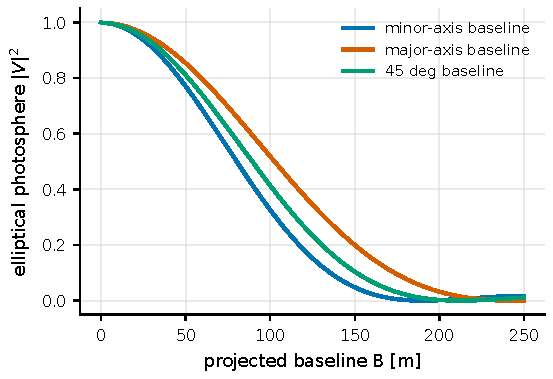
\includegraphics[width=0.82\linewidth]{figures/generated/chapter_10/ch10_rotation_oblateness.pdf}
\caption{快速自转椭圆光球在不同基线方向上的 \(|V|^2\)。参数取 \(\gamma\) Cas 量级的轴比 \(1.28\) 和 \(416~{\rm nm}\) 波长。沿不同位置角投影时，有效角直径不同，因此同一基线长度给出的相关强度也不同；这一几何效应使 SII 能测 photosphere oblateness。}
\label{fig:chapter-10-rotation}
\end{figure}

\Needspace{13\baselineskip}
双星在可见度空间中产生振荡。若两颗星本身未分辨，角分离向量为 \({\boldsymbol d}\)，次星与主星流量比为 \(f\)，则
\begin{equation}
  |V_{\rm bin}|^2=
  \frac{1+f^2+2f\cos(2\pi{\boldsymbol u}\cdot{\boldsymbol d})}
       {(1+f)^2}.
  \label{eq:ch10-binary}
\end{equation}
\begin{formulaexplain}
\(|V_{\rm bin}|^2\) 是未分辨双星的平方可见度；\(f\) 是流量比，\({\boldsymbol u}\) 是空间频率，\({\boldsymbol d}\) 是角分离向量。余弦项让双星在基线空间产生振荡。
\end{formulaexplain}
\({\boldsymbol u}={\boldsymbol B}_\perp/\lambda\)，\({\boldsymbol d}\) 用弧度。振荡周期给出沿基线方向的分离，振幅给出流量比；若每颗星被部分分辨，还要把各自的圆盘可见度乘进去。Narrabri 目录中一些目标后来被识别为双星或多星，现代 SII 多基线阵列可以把双星轨道、角直径和亮度比联合拟合，再与径向速度结合得到质量 \citep{1970MNRAS.148..103H,1974MNRAS.167..121H,2012MNRAS.419..172N}。

\begin{figure}[tbp]
\centering
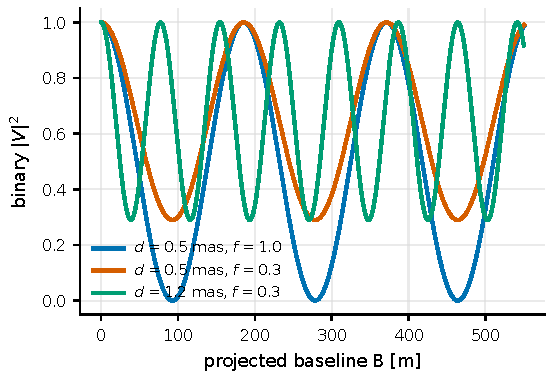
\includegraphics[width=0.82\linewidth]{figures/generated/chapter_10/ch10_binary_visibility.pdf}
\caption{未分辨双星的 \(|V|^2\) 振荡。角分离越大，随基线振荡越快；流量比越接近 1，振荡幅度越大。真实双星还需要加入两颗星的有限角直径、轨道位置角和多波长流量比。}
\label{fig:chapter-10-binary}
\end{figure}

表面结构比双星更难，因为 \(|V|^2\) 缺少相位。星斑、对流单元、非径向脉动和 Be 星盘都会引入非轴对称信号；只用一个圆盘或双星模型可能给出看似漂亮但物理错误的拟合。多基线、多夜晚、多波长和谱线通道可以破除一部分退化。模拟研究显示，Cherenkov 望远镜阵列的基线数量和覆盖范围有机会重建直径、扁率、双星结构和大尺度表面特征，但复杂图像仍需要先验或联合振幅干涉数据 \citep{2012MNRAS.419..172N,2013MNRAS.430.3187R,2012NewAR..56..143D}。

\section{时间变化和谱线通道怎样扩展恒星图像}

造父变星把角直径测量连接到距离标尺。Baade--Wesselink 类方法比较角半径变化和视向速度积分：
\begin{equation}
  \Delta\theta(t)=\frac{2}{d}
  \int p\,[v_r(t)-v_\gamma]\,{\rm d}t .
  \label{eq:ch10-baade-wesselink}
\end{equation}
\begin{formulaexplain}
\(\Delta\theta(t)\) 是角直径变化，\(d\) 是距离，\(v_r-v_\gamma\) 是扣除系统速度后的径向速度，\(p\) 是投影因子。它把脉动速度积分和角半径变化联系起来。
\end{formulaexplain}
\(d\) 是距离，\(v_r\) 是径向速度，\(v_\gamma\) 是系统速度，\(p\) 是把观测径向速度转换为真实脉动速度的投影因子。角直径曲线和速度曲线相位匹配后可求距离。系统误差来自 \(p\) 因子、边缘昏暗、伴星污染、周期变化和大气速度梯度。明亮造父在可见光 SII 中尤其有吸引力，因为它们既亮又有可预测的半径变化 \citep{1997A&A...320..799F,2007A&A...476...73F,2012NewAR..56..143D}。

Be 星和 Wolf--Rayet 星把连续谱和谱线空间结构分开。若窄带滤波器覆盖一条发射线，观测可见度是连续谱和线区的通量加权和：
\begin{equation}
  V_{\rm obs}=
  \frac{F_{\rm cont}V_{\rm cont}+F_{\rm line}V_{\rm line}}
       {F_{\rm cont}+F_{\rm line}} .
  \label{eq:ch10-line-visibility}
\end{equation}
\begin{formulaexplain}
\(V_{\rm obs}\) 是窄带观测到的可见度；连续谱和谱线分量按通量 \(F_{\rm cont},F_{\rm line}\) 加权。若连续谱已标定，就能反推出谱线形成区的空间尺度。
\end{formulaexplain}
若连续谱光球已由邻近谱带标定，就可以反推出谱线形成区的 \(V_{\rm line}\)，进而约束盘半径、倾角或星风几何。对于快速旋转 Be 星，H\(\alpha\) 谱线给盘，蓝光连续谱给光球；\(\gamma\) Cas 的例子表明，SII 可以直接测到光球扁率，而红外或 H\(\alpha\) 干涉则补充盘的几何 \citep{2025ApJ...995..191A}。

自然激光和受激谱线在恒星环境中也可能出现，尤其是 \(\eta\) Carinae 这类强辐射场和密集气体团块共存的系统。对这类目标，普通谱线强度不足以证明受激辐射；需要同时看线宽、空间位置、泵浦通道、偏振和谱线通道的 \(g^{(2)}\)。第 \ref{chap:09} 章讨论的自然激光诊断可转化为具体目标选择 \citep{2004A&A...428..497J,2005NewA...10..361J,2008AIPC..984..216D}。

